\documentclass[border=1pt]{standalone}
% ---------------------------------------------------------------------------
% Shared style for the MOSAIC / CRYSTAL TOMM figures.
% Compile each fig_*.tex with LuaLaTeX (standalone). Sized for acmart
% "acmsmall" (TOMM): \textwidth = 13.9 cm, so every figure is drawn at
% final size and is included with width=\textwidth (no rescaling of text).
% Fonts: Libertinus Sans + Inconsolata (acmart uses Libertine + Inconsolata).
% ---------------------------------------------------------------------------
\usepackage{fontspec}
\setmainfont{LibertinusSans}[Path=fonts/, Extension=.otf,
  UprightFont=*-Regular, BoldFont=*-Bold, ItalicFont=*-Italic]
\setmonofont{Inconsolata}[Path=fonts/, Extension=.otf,
  UprightFont=*-Regular, BoldFont=*-Bold, Scale=0.98]
\usepackage{unicode-math}
\setmathfont{LibertinusMath-Regular.otf}[Path=fonts/]

\usepackage{tikz}
\usetikzlibrary{positioning,fit,calc,arrows.meta,backgrounds,
  shapes.misc,shapes.geometric,decorations.pathreplacing,patterns.meta}

% Okabe-Ito palette (colour-blind safe) + tints -------------------------------
\definecolor{oiBlue}{HTML}{0072B2}
\definecolor{oiOrange}{HTML}{E69F00}
\definecolor{oiSky}{HTML}{56B4E9}
\definecolor{oiGreen}{HTML}{009E73}
\definecolor{oiVerm}{HTML}{D55E00}
\definecolor{oiPurple}{HTML}{CC79A7}
\definecolor{oiYellow}{HTML}{F0E442}
\definecolor{ink}{HTML}{1A1A1A}
\definecolor{muted}{HTML}{5C5C5C}
\definecolor{rule}{HTML}{9A9A9A}

\definecolor{oursFill}{HTML}{DDEBF7}
\definecolor{oursDraw}{HTML}{0072B2}
\definecolor{modFill}{HTML}{FCEFD2}
\definecolor{modDraw}{HTML}{B57600}
\definecolor{upFill}{HTML}{F1F1F1}
\definecolor{upDraw}{HTML}{7D7D7D}
\definecolor{failFill}{HTML}{FBE3D6}
\definecolor{okFill}{HTML}{D9F0E8}

% Sequence colours (as in the packetization study)
\definecolor{seqSOL}{HTML}{0072B2}
\definecolor{seqTHA}{HTML}{009E73}
\definecolor{seqLON}{HTML}{CC79A7}

% Typography -----------------------------------------------------------------
\newcommand{\figfont}{\fontsize{7.5}{9}\selectfont}
\newcommand{\smallfig}{\fontsize{6.5}{7.8}\selectfont}
\newcommand{\tinyfig}{\fontsize{6}{7.2}\selectfont}
\newcommand{\code}[1]{{\ttfamily #1}}

% Provenance encoding: colour AND line style (grayscale safe) ------------------
%  ours      = new component written by us      (blue, solid 0.9 pt)
%  modified  = upstream component we patched    (orange, dashed 0.8 pt)
%  upstream  = used unmodified / third party    (grey, solid 0.45 pt)
\tikzset{
  base/.style={rectangle, rounded corners=1.6pt, align=center,
    inner xsep=3pt, inner ysep=2.6pt, font=\figfont, text=ink,
    execute at begin node={\hyphenpenalty=10000\exhyphenpenalty=10000}},
  ours/.style={base, fill=oursFill, draw=oursDraw, line width=0.9pt},
  mod/.style={base, fill=modFill, draw=modDraw, line width=0.8pt,
    dash pattern=on 2.6pt off 1.4pt},
  up/.style={base, fill=upFill, draw=upDraw, line width=0.45pt},
  dead/.style={base, fill=white, draw=oiVerm, line width=0.6pt,
    dash pattern=on 1.2pt off 1.2pt, text=oiVerm},
  note/.style={font=\smallfig, text=muted, align=left,
    execute at begin node={\hyphenpenalty=10000\exhyphenpenalty=10000}},
  lab/.style={font=\smallfig\itshape, text=muted},
  zone/.style={draw=rule, line width=0.45pt, rounded corners=3pt,
    dash pattern=on 0.6pt off 1.1pt},
  zonetitle/.style={font=\figfont\bfseries, text=ink, anchor=west,
    inner xsep=2pt, inner ysep=1pt, fill=white, xshift=2.5mm},
  flow/.style={-{Stealth[length=4pt,width=3.2pt]}, line width=0.65pt,
    draw=ink},
  dflow/.style={flow, dash pattern=on 2pt off 1.4pt},
  ctrl/.style={-{Stealth[length=3.4pt,width=2.8pt]}, line width=0.5pt,
    draw=muted},
  failflow/.style={-{Stealth[length=4pt,width=3.2pt]}, line width=0.6pt,
    draw=oiVerm, dash pattern=on 1.4pt off 1.2pt},
  stepc/.style={circle, fill=ink, text=white, inner sep=0pt,
    minimum size=8.5pt, font=\tinyfig\bfseries},
  tag/.style={font=\tinyfig\bfseries, inner sep=1pt},
}

% Legend for the provenance encoding -------------------------------------------
\newcommand{\provlegend}[1]{% #1 = anchor coordinate (north west)
  \begin{scope}[shift={(#1)}]
    \node[ours, minimum width=6mm, minimum height=2.6mm, inner sep=0pt]
      (lg1) at (0,0) {};
    \node[anchor=west, font=\smallfig] at (lg1.east) {new (this work)};
    \node[mod, minimum width=6mm, minimum height=2.6mm, inner sep=0pt]
      (lg2) at (2.6,0) {};
    \node[anchor=west, font=\smallfig] at (lg2.east) {upstream, patched by us};
    \node[up, minimum width=6mm, minimum height=2.6mm, inner sep=0pt]
      (lg3) at (6.2,0) {};
    \node[anchor=west, font=\smallfig] at (lg3.east) {upstream / third party, unmodified};
  \end{scope}}

\usepackage{pgfplots}
\pgfplotsset{compat=1.18}
\newcommand{\bx}[2]{{\bfseries #1\par}\vspace{0.6pt}{\smallfig #2\par}}
\begin{document}
\figfont
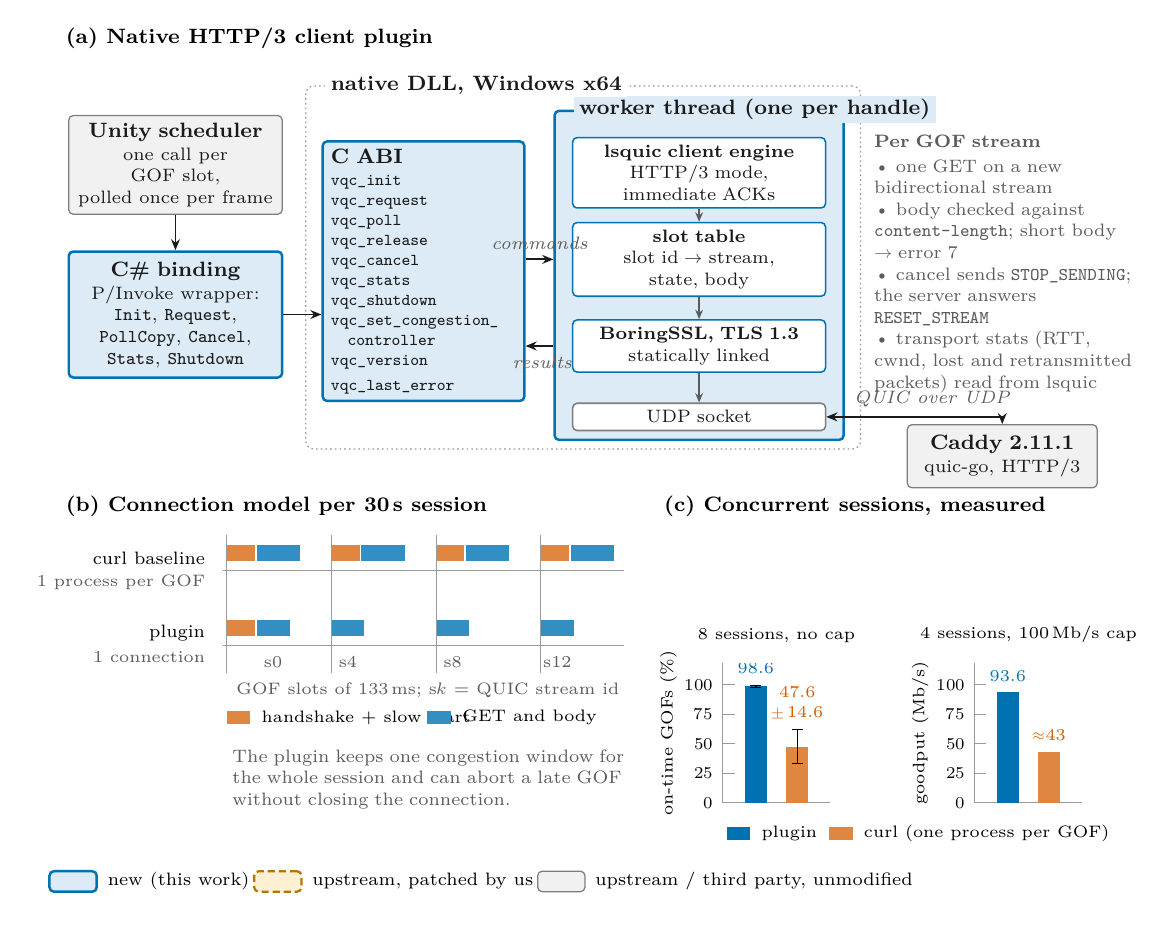
\begin{tikzpicture}[x=1cm,y=1cm]
  \tikzset{api/.style={font=\tinyfig\ttfamily, text=ink, align=left, inner sep=1pt},
           panel/.style={font=\figfont\bfseries, anchor=north west, inner sep=0pt},
           inner/.style={base, fill=white, draw=oursDraw, line width=0.55pt, font=\smallfig}}

  \node[panel] at (0,10.4) {(a) Native HTTP/3 client plugin};

  % ---------------- managed side ----------------
  \node[up, text width=2.5cm, minimum height=0.95cm] (ctl) at (1.4,8.65)
    {\bx{Unity scheduler}{one call per GOF slot,\\polled once per frame}};
  \node[ours, text width=2.5cm, minimum height=1.6cm] (cs) at (1.4,6.75)
    {\bx{C\# binding}{P/Invoke wrapper:\\\code{Init}, \code{Request},\\\code{PollCopy}, \code{Cancel},\\\code{Stats}, \code{Shutdown}}};
  \draw[flow] (ctl) -- (cs);

  % ---------------- C ABI ----------------
  \node[ours, text width=2.35cm, minimum height=3.1cm, align=left] (abi) at (4.55,7.3)
    {{\bfseries C ABI}\par\vspace{1pt}
     {\tinyfig\ttfamily vqc\_init\\vqc\_request\\vqc\_poll\\vqc\_release\\vqc\_cancel\\vqc\_stats\\vqc\_shutdown\\vqc\_set\_congestion\_\\\hspace*{6pt}controller\\vqc\_version\\vqc\_last\_error}};
  \draw[flow] (cs.east) -- (abi.west |- cs.east);

  % ---------------- worker thread ----------------
  \node[inner, text width=3.0cm] (eng) at (8.05,8.55)
    {{\bfseries lsquic client engine}\par HTTP/3 mode, immediate ACKs};
  \node[inner, text width=3.0cm] (slot) at (8.05,7.45)
    {{\bfseries slot table}\par slot id $\rightarrow$ stream, state, body};
  \node[inner, text width=3.0cm] (tls) at (8.05,6.35)
    {{\bfseries BoringSSL, TLS 1.3}\par statically linked};
  \node[inner, text width=3.0cm, draw=upDraw] (udp) at (8.05,5.45) {UDP socket};
  \draw[ctrl] (eng) -- (slot); \draw[ctrl] (slot) -- (tls); \draw[ctrl] (tls) -- (udp);
  \begin{scope}[on background layer]
    \node[ours, fit=(eng)(slot)(tls)(udp), inner sep=2.2mm, yshift=1.1mm] (zw) {};
  \end{scope}
  \node[zonetitle, fill=oursFill] at (zw.north west) {worker thread (one per handle)};
  \draw[flow] (abi.east |- slot.west) -- (zw.west |- slot.west) node[midway, above, lab] {commands};
  \draw[flow] (zw.west |- tls.west) -- (abi.east |- tls.west) node[pos=0.4, below, lab] {results};

  % ---------------- per-stream behaviour ----------------
  \node[note, text width=3.3cm, anchor=north west, execute at begin node={\hyphenpenalty=10000}] (beh) at (10.15,9.15)
    {\textbf{Per GOF stream}\\[1pt]
     \textbullet\ one GET on a new bidirectional stream\\
     \textbullet\ body checked against \code{content-length}; short body $\rightarrow$ error 7\\
     \textbullet\ cancel sends \code{STOP\_SENDING}; the server answers \code{RESET\_STREAM}\\
     \textbullet\ transport stats (RTT, cwnd, lost and retransmitted packets) read from lsquic};

  \node[up, text width=2.2cm, minimum height=0.8cm] (srv) at (11.9,4.95)
    {\bx{Caddy 2.11.1}{quic-go, HTTP/3}};
  \draw[flow, {Stealth[length=4pt,width=3.2pt]}-{Stealth[length=4pt,width=3.2pt]}] (udp.east) -| (srv.north)
    node[pos=0.3, above, lab] {QUIC over UDP};

  \begin{scope}[on background layer]
    \node[zone, fit=(abi)(zw), inner sep=2.0mm, yshift=1mm] (zdll) {};
  \end{scope}
  \node[zonetitle] at ($(zdll.north west)+(0,0.0)$) {native DLL, Windows x64};

  % ======================= (b) connection model ==============================
  \node[panel] at (0,4.45) {(b) Connection model per 30\,s session};
  \tikzset{hs/.style={fill=oiVerm!75, draw=none},
           get/.style={fill=oiBlue!80, draw=none},
           axisl/.style={draw=rule, line width=0.4pt}}
  % curl baseline
  \node[font=\smallfig, anchor=east] at (1.9,3.65) {curl baseline};
  \node[font=\tinyfig, text=muted, anchor=east] at (1.9,3.35) {1 process per GOF};
  \draw[axisl] (2.0,3.5) -- (7.1,3.5);
  \foreach \x in {2.05,3.38,4.71,6.04}{
    \fill[hs] (\x,3.62) rectangle ++(0.36,0.2);
    \fill[get] (\x+0.38,3.62) rectangle ++(0.55,0.2);}
  % plugin
  \node[font=\smallfig, anchor=east] at (1.9,2.7) {plugin};
  \node[font=\tinyfig, text=muted, anchor=east] at (1.9,2.4) {1 connection};
  \draw[axisl] (2.0,2.55) -- (7.1,2.55);
  \fill[hs] (2.05,2.67) rectangle ++(0.36,0.2);
  \foreach \x/\s in {2.43/0,3.38/4,4.71/8,6.04/12}{
    \fill[get] (\x,2.67) rectangle ++(0.42,0.2);
    \node[font=\tinyfig, text=muted, anchor=north] at (\x+0.21,2.53) {s\s};}
  % ticks: GOF slots
  \foreach \i/\x in {0/2.05,1/3.38,2/4.71,3/6.04}{
    \draw[rule, line width=0.3pt] (\x,2.2) -- (\x,3.95);}
  \node[font=\tinyfig, text=muted, anchor=north west] at (2.05,2.2) {GOF slots of 133\,ms; s$k$ = QUIC stream id};
  % legend
  \fill[hs] (2.05,1.55) rectangle ++(0.3,0.16);
  \node[font=\tinyfig, anchor=west] at (2.37,1.63) {handshake + slow start};
  \fill[get] (4.6,1.55) rectangle ++(0.3,0.16);
  \node[font=\tinyfig, anchor=west] at (4.92,1.63) {GET and body};
  \node[note, text width=5.1cm, anchor=north west] at (2.0,1.35)
    {The plugin keeps one congestion window for the whole session and can abort a late GOF without closing the connection.};

  % ======================= (c) measured comparison ===========================
  \node[panel] at (7.6,4.45) {(c) Concurrent sessions, measured};
  \begin{axis}[at={(8.35cm,0.55cm)}, anchor=south west,
      width=2.95cm, height=3.35cm, scale only axis=false,
      ybar, bar width=8pt, bar shift=0pt, ymin=0, ymax=118, xmin=-0.8, xmax=1.8,
      xtick=\empty, ytick={0,25,50,75,100},
      axis lines*=left, axis line style={draw=rule},
      tick style={draw=rule}, tick label style={font=\tinyfig},
      ylabel={on-time GOFs (\%)}, ylabel style={font=\tinyfig, yshift=-4pt},
      title={8 sessions, no cap}, title style={font=\tinyfig, yshift=-2pt},
]
    \addplot[fill=oiBlue, draw=none, error bars/.cd, y dir=both, y explicit,
        error bar style={line width=0.5pt}]
      coordinates {(0,98.6) +- (0,0.6)};
    \addplot[fill=oiVerm!75, draw=none, error bars/.cd, y dir=both, y explicit,
        error bar style={line width=0.5pt}]
      coordinates {(1,47.6) +- (0,14.6)};
    \node[font=\tinyfig, anchor=south, text=oiBlue] at (axis cs:0,100.5) {98.6};
    \node[font=\tinyfig, anchor=south, text=oiVerm, align=center] at (axis cs:1,63) {47.6\\$\pm$\,14.6};
  \end{axis}
  \begin{axis}[at={(11.55cm,0.55cm)}, anchor=south west,
      width=2.95cm, height=3.35cm,
      ybar, bar width=8pt, bar shift=0pt, ymin=0, ymax=118, xmin=-0.8, xmax=1.8,
      xtick=\empty, ytick={0,25,50,75,100},
      axis lines*=left, axis line style={draw=rule},
      tick style={draw=rule}, tick label style={font=\tinyfig},
      ylabel={goodput (Mb/s)}, ylabel style={font=\tinyfig, yshift=-4pt},
      title={4 sessions, 100\,Mb/s cap}, title style={font=\tinyfig, yshift=-2pt},
]
    \addplot[fill=oiBlue, draw=none] coordinates {(0,93.6)};
    \addplot[fill=oiVerm!75, draw=none] coordinates {(1,43)};
    \node[font=\tinyfig, anchor=south, text=oiBlue] at (axis cs:0,94.5) {93.6};
    \node[font=\tinyfig, anchor=south, text=oiVerm] at (axis cs:1,44) {$\approx$43};
  \end{axis}
  \fill[oiBlue] (8.4,0.08) rectangle ++(0.3,0.16);
  \node[font=\tinyfig, anchor=west] at (8.72,0.16) {plugin};
  \fill[oiVerm!75] (9.7,0.08) rectangle ++(0.3,0.16);
  \node[font=\tinyfig, anchor=west] at (10.02,0.16) {curl (one process per GOF)};

  \provlegend{0.1,-0.45}
\end{tikzpicture}
\end{document}
